% !TEX encoding = UTF-8 Unicode
% -*- coding: UTF-8; -*-
\ifdefined\ishandout
\documentclass[handout]{beamer}
\else
\documentclass[11pt]{beamer}
\fi

\usepackage[frenchb]{babel}
\usepackage[T1]{fontenc}
\usepackage[utf8]{inputenc}
\usepackage{hyperref}
\usepackage{multirow}
\usepackage{listings}
\usepackage{fancyvrb}
\usepackage{tikz}
\usepackage{framed}
\usepackage{algorithm}
\usepackage{algorithmic}
\usepackage{xcolor}
\usepackage{color, colortbl}
\ifdefined\ishandout
\usepackage{handoutWithNotes}
\fi
\usepackage{slashbox}
\usepackage{amsmath}
\usepackage{bm}
\usepackage{hhline}
\usepackage{xmpmulti}

\usetikzlibrary{shapes.geometric}
\usetikzlibrary{positioning}
\usetikzlibrary{shapes.arrows, chains}
\usetikzlibrary{arrows,calc}
\usetikzlibrary{shapes.multipart}
\usepackage{array}
\usetheme{Boadilla}

\usefonttheme[onlymath]{serif}

\newcommand{\R}{\mathbb{R}}
\newcommand{\C}{\mathbb{C}}
\newcommand{\N}{\mathbb{N}}
\newcommand{\Z}{\mathbb{Z}}
\newcommand{\E}{\mathbb{E}}
\newcommand{\Var}{\text{Var}}
\newcommand{\Cov}{\text{Cov}}
\ifdefined\ishandout
\pgfpagesuselayout{3 on 1 with notes}[a4paper,border shrink=5mm]
\usecolortheme{dove}
\else
%\usecolortheme{dolphin}
\usecolortheme{beaver}
\fi


\lstnewenvironment{codeC}
{ \lstset{language=C,
    otherkeywords={printf,scanf}}
}
{}

\ifdefined\ishandout
\definecolor{mygreen}{rgb}{0,0,0}
\definecolor{mymauve}{rgb}{0,0,0}
\definecolor{myblue}{rgb}{0,0,0}
\else
\definecolor{mygreen}{rgb}{0,0.6,0}
\definecolor{mymauve}{rgb}{0.58,0,0.82}
\definecolor{myblue}{rgb}{0,0,1}

\fi

%% Notes
%\setbeameroption{show only notes}


\definecolor{mygray}{rgb}{0.5,0.5,0.5}

\lstset{ language=Python,%
  backgroundcolor=\color{white},   % choose the background color; you must add \usepackage{color} or \usepackage{xcolor}
  basicstyle=\footnotesize,        % the size of the fonts that are used for the code
  breakatwhitespace=false,         % sets if automatic breaks should only happen at whitespace
  breaklines=true,                 % sets automatic line breaking
  captionpos=b,                    % sets the caption-position to bottom
  commentstyle=\color{mygreen},    % comment style
  deletekeywords={...},            % if you want to delete keywords from the given language
  escapeinside={\%*}{*)},          % if you want to add LaTeX within your code
  extendedchars=true,              % lets you use non-ASCII characters; for 8-bits encodings only, does not work with UTF-8
  frame=tb,	                   % adds a frame around the code
  keepspaces=true,                 % keeps spaces in text, useful for keeping indentation of code (possibly needs columns=flexible)
  keywordstyle=\color{blue},       % keyword style
  otherkeywords={*,...},           % if you want to add more keywords to the set
  numbers=none,                    % where to put the line-numbers; possible values are (none, left, right)
  numbersep=5pt,                   % how far the line-numbers are from the code
  numberstyle=\tiny\color{mygray}, % the style that is used for the line-numbers
  rulecolor=\color{black},         % if not set, the frame-color may be changed on line-breaks within not-black text (e.g. comments (green here))
  showspaces=false,                % show spaces everywhere adding particular underscores; it overrides 'showstringspaces'
  showstringspaces=false,          % underline spaces within strings only
  showtabs=false,                  % show tabs within strings adding particular underscores
  stepnumber=2,                    % the step between two line-numbers. If it's 1, each line will be numbered
  stringstyle=\color{mymauve},     % string literal style
  tabsize=3,	                   % sets default tabsize to 2 spaces
  title=\lstname                   % show the filename of files included with \lstinputlisting; also try caption instead of title
}
%\lstset{language=Python,
% breakatwhitespace=false,         % sets if automatic breaks should only happen at whitespace
%  breaklines=true,                 % sets automatic line breaking
%  captionpos=b,                
%%commentstyle=\itshape\color{mymauve},
%%keywordstyle=\bfseries\color{myblue},
%numbers=left,                    % where to put the line-numbers; possible values are (none, left, right)
%  numbersep=8pt,                   % how far the line-numbers are from the code
%  numberstyle=\tiny\color{mygray}, % the style that is used for the line-numbers
%%  rulecolor=\color{black},         % if not set, the frame-color may be changed on line-breaks within not-black text (e.g. comments (green here))
%  showspaces=false,                % show spaces everywhere adding particular underscores; it overrides 'showstringspaces'
%%  showstringspaces=false,          % underline spaces within strings only
%  showtabs=false,                  % show tabs within strings adding particular underscores
%  stepnumber=2,                    % the step between two line-numbers. If it's 1, each line will be numbered
%%  stringstyle=\color{mygreen},     % string literal style
%  tabsize=2 
%}
\ifdefined\ishandout
\newcommand{\red}{\textbf}
\else
\newcommand{\red}{\textcolor{red}}
\fi
%\newcommand \emph
%Default size : 12.8 cm * 9.6 cm

\newcommand{\tmark}[1]{\tikz[remember picture, baseline=-.5ex]{\coordinate(#1);}}

\ifdefined\ishandout
\newenvironment<>{codeblock}[1]{%begin
  \setbeamercolor{block title}{fg=black,bg=lightgray!80}%
  \begin{block}{#1}}
  % \begin{codeC}}
  %  {\end{codeC}
{  
\end{block}}

\newenvironment<>{termblock}[1]{
    \setbeamercolor{block title}{fg=black,bg=lightgray!90}%
    \begin{block}{#1}
}
%     \begin{Verbatim}}
{%\end{Verbatim}
\end{block}
}

\definecolor{bluegreen}{RGB}{0,0,0}
%\definecolor{bluegreen}{rgb}{0,0.6,0.8}
\else

\newenvironment<>{codeblock}[1]{%begin
  \setbeamercolor{block title}{fg=darkgray,bg=yellow}%
  \begin{block}{#1}}
  % \begin{codeC}}
  %  {\end{codeC}
{  
\end{block}}

\newenvironment<>{termblock}[1]{
    \setbeamercolor{block title}{fg=white,bg=lightgray}%
    \begin{block}{#1}}
%     \begin{Verbatim}}
{%\end{Verbatim}
\end{block}
}

\definecolor{bluegreen}{RGB}{0,149,182}
%\definecolor{bluegreen}{rgb}{0,0.6,0.8}
\fi

%\newcommand{\output}[1]{
\setbeamertemplate{navigation symbols}{}
\newcommand{\bvrb}{\Verb[commandchars=£µ§,formatcom=\color{bluegreen}]}
\newcommand{\footvrb}{\footnotesize\Verb}
\newcommand{\vrbalert}[2][]{\visible<#1>{#2}}
%%% Commande pour les listes/arbres
\newcommand{\mvide}{\nodepart{one} \nodepart{two}}
\newcommand{\tvide}{\nodepart{one} \nodepart{two} \nodepart{three}}
\newcommand{\rref}[1][]{\hfill{\scriptsize\textit{#1}}}


\newcommand{\odif}[2]{\frac{d #1}{d #2}} 
%%Fin des commandes pour les listes/arbres.
\newcommand{\gooditem}[1]{\setbeamercolor{item}{fg=green}\item #1} 
\newcommand{\pooritem}[1]{\setbeamercolor{item}{fg=red}\item #1} 
\setbeamerfont{caption}{size=\scriptsize}

%%% Paramètres du cours (à régler)
%Numéro du cours
\newcommand{\nb}{1}

\title[lagrangian assimilation]{Assimilation of non-conventional observations. Application to the estimating of ocean surface currents.}
\author[J. Brajard]{julien.brajard@upmc.fr}
\institute[LOCEAN/UPMC]{LOCEAN-UPMC}
\date{29 May 2017}
\begin{document}
\tikzstyle{every picture}+=[remember picture]
%%%%%%%%%%%%%%%%%%%%% SLIDES DE TITRE
\begin{frame}
\titlepage
%\centering{
%\url{http://australe.upmc.fr} (onglet EPU-C5-IGE Info Gen)}
\end{frame}

%%%%%%%%%%%%%%%%%%%%
\begin{frame}
\frametitle{LOCEAN institute}
\begin{figure}

\includegraphics[height=0.1\textheight]{../../fig/logo-locean.png}
\end{figure}
Laboratory in University Pierre et Marie Curie (shorlty Sorbonne
Université) with scientific thematics :
\begin{itemize}
\item Physical oceanography
\item Marine bio-geochemistry
\item Climate
\item Paleocenography
\item ...
\end{itemize}
Using a wide spectra of approaches:
\begin{itemize}
\item Numerical modelling
\item Statistical modelling
\item Observations (campaigns, or autonomous plateforms)
\item Remote-sensing
\end{itemize}
\end{frame}
%%%%%%%%%%%%%%%%%%%%%
\begin{frame}
\frametitle{Data assimilation}
\begin{block}{Objective}
Optimally combine output of an numerical model and some observations
\end{block}
\begin{tikzpicture}
\draw[thick,->](-0.2,0)--(10,0) node[below]{$time$};
\draw[thick,->](0,-0.2)--(0,5) node[left]{$x$};
\draw[red,very thick] plot [smooth] 
coordinates {(0,1)  (1,1)  (3,2) (5,0.5) (7,4) (9,3) } ;
\draw plot [mark=*, mark size=5pt, only marks, mark options={color=red}]
coordinates{(0,1)} node [left,xshift=-0.5em]{\textcolor{red}{$x^b$}};
\draw <2-> plot [mark=*, mark size=3pt, only marks, mark options={color=blue}]
coordinates {(0.5,2) (3,3) (4,0.5) (6,4.5) (8,3)};
\draw <3-> [magenta,very thick] plot [smooth] 
coordinates {(0,2)  (1,2.5)  (3,2.8) (4.6,0.1) (6,4) (9,2.5) } ;
\draw <3-> plot [mark=*, mark size=5pt, only marks, mark options={color=magenta}]
coordinates{(0,2)} node [left,xshift=-0.5em]{\textcolor{magenta}{$x^a$}};
\draw (0.1,5.4) node [anchor=west] {\textcolor{red} {$-$ background}};
\draw <2-> (0.1,4.8) node [anchor=west] {\textcolor{blue} {$\bullet$ observations}};
\draw <3-> (0.1,4.2) node[anchor=west]  {\textcolor{magenta} {$-$ analyze}};
\end{tikzpicture}
\end{frame}


%%%%%%%%%%%%%%%%%%%%%%
\begin{frame}
\frametitle{Some equations...}
The basics ingredients for data assimilation are :
\begin{itemize}[<+->]
\item A state vector: $\bm{x_k}$
\item A dynamical model (with error): $\bm{x_k} = M_k(\bm{x_{k-1}}) +
  \bm{w_k}$
\item Some observations at time $\bm{k}$: $\bm{y_k} = H_k(\bm{x_k}) +
  \bm{v_k}$
\item An background state (often at time 0): $\bm{x^b_0} = \bm{x_0} +
  \bm{e_k}$
\item Error statistics: 
\begin{itemize}
\item $\E[\bm{w_kw_k^T}] = \bm{Q_k}$
\item $\E[\bm{v_kv_k^T}] = \bm{R_k}$
\item $\E[\bm{e_ke_k^T}] = \bm{B_k}$
\end{itemize}
\end{itemize}
\pause
\begin{alertblock}{Objective}
Estimate the more likely state $\bm{x_k^a}$ knowing
$M$,$H$,$\bm{y}$,$\bm{x^b}$,$\bm{Q}$,$\bm{R}$ and $\bm{B}$
\end{alertblock}
\end{frame}

%%%%%%%%%%%%%%%%%%%%%%
\begin{frame}
\frametitle{Example of "non-conventional" observations}
\begin{columns}[t]
\column{.5\textwidth}
Remote sensing
\begin{figure}
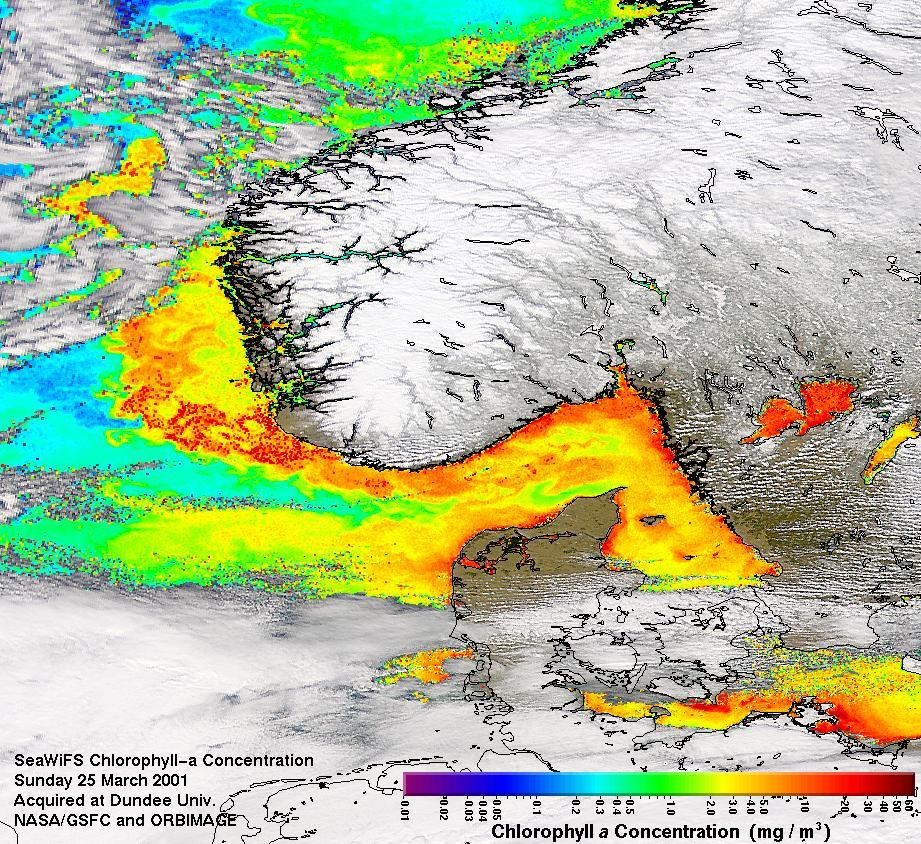
\includegraphics[width=\textwidth]{./fig/chla-norway.jpg}
\caption{chlorophylle-a concentration }
\end{figure}
\pause
\column{.5\textwidth}
Lagrangian observations
\begin{figure}
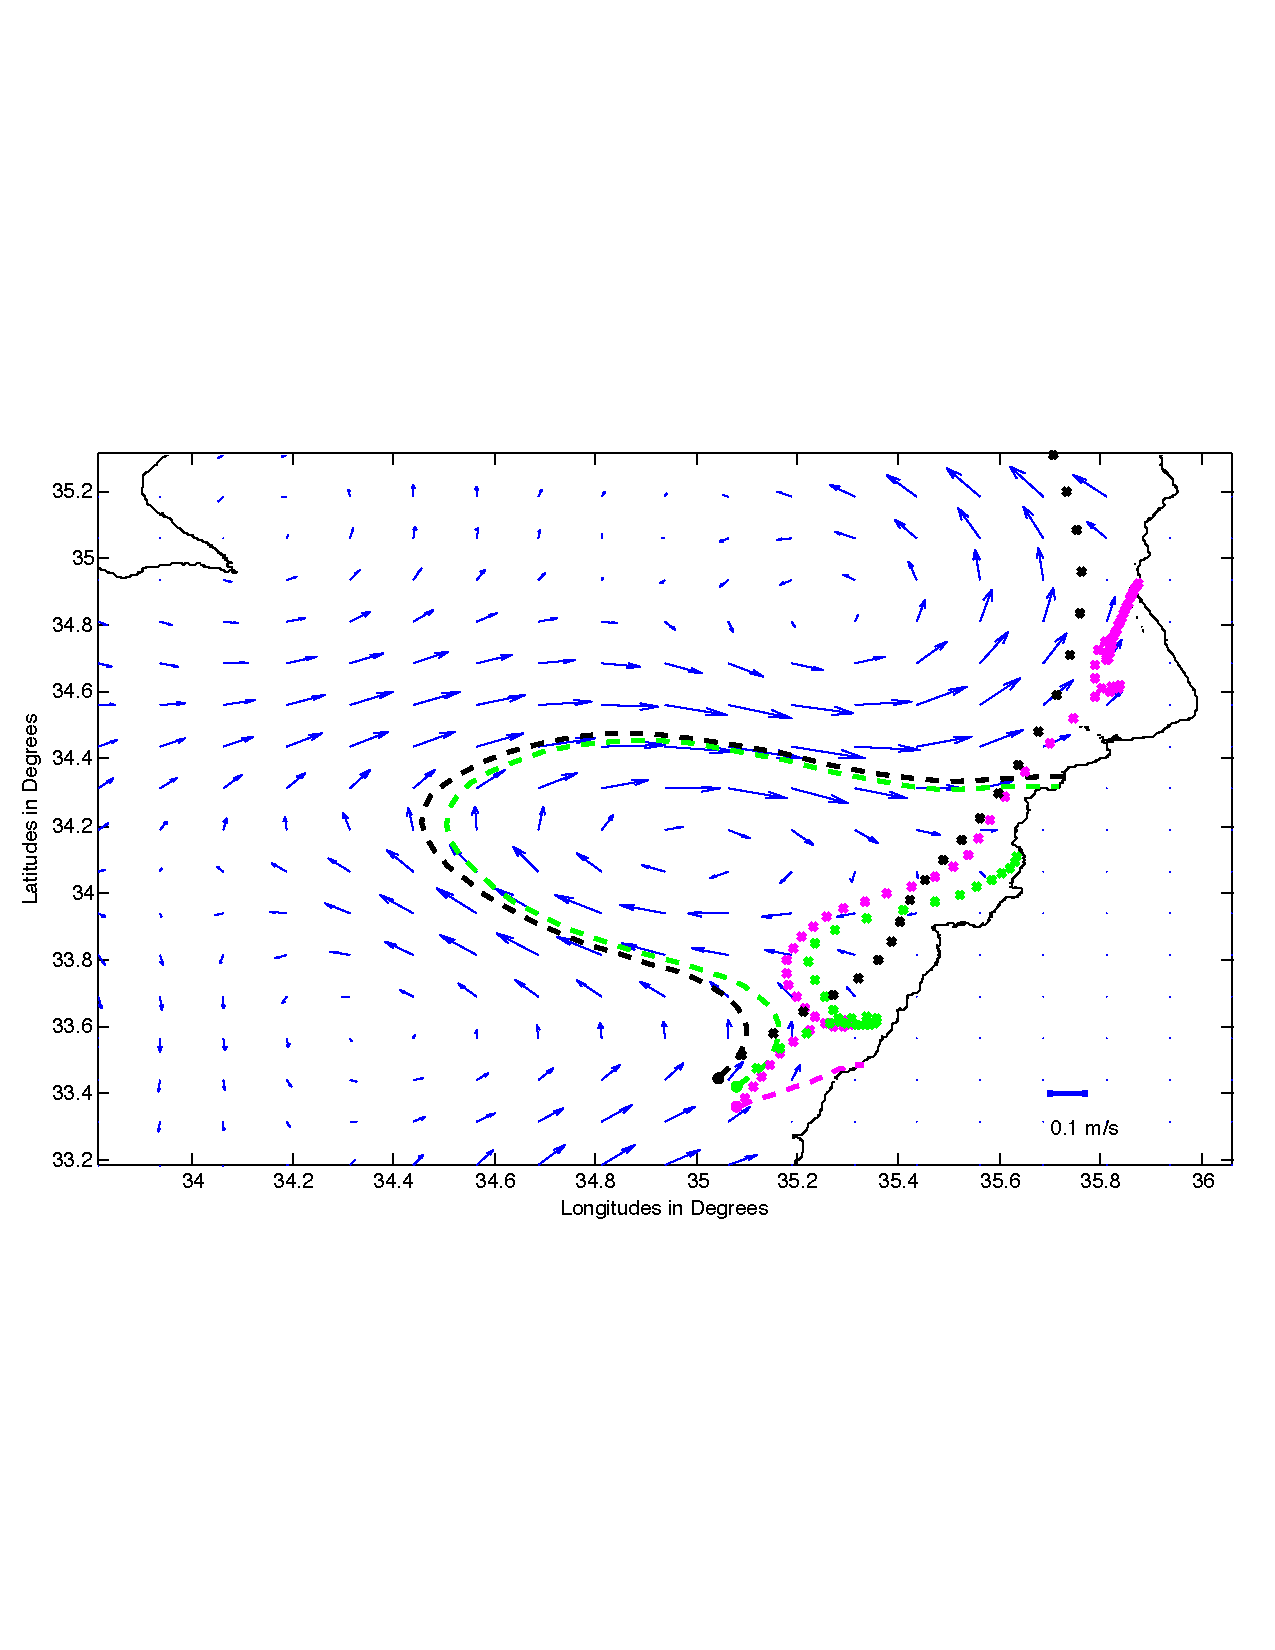
\includegraphics[width=\textwidth]{./fig/RealvsSimulatedTraj.pdf}
\caption{Drifters deployed on 29 Aug. 2013 (x) versus trajectories
  simulated using altimetry field (-)}
\end{figure}

\end{columns}
\end{frame}


%%%%%%%%%%%%%%%%%%%%%%
\begin{frame}
\frametitle{Position of the problem}
\begin{columns}
\column{.5\textwidth}
  \begin{figure}
 \begin{center}
 \includegraphics[width=\textwidth]{./fig/chart1.png}
\end{center}
 \end{figure}
 \column{.5\textwidth}
 \begin{figure}
 \begin{center}
\includegraphics[width=\textwidth]{./fig/Euler_LagrangeNew.png}
\end{center}
 \end{figure}
 \end{columns}
 
\begin{itemize}
\item $\mathcal{M}$ is a parametrization of non-geostrophic effects (wind)
\item $\mathcal{G}$ is the advection operator solving
  $\odif{\vec{r}}{t} =\vec{U}(\vec{r}(t),t)$
\end{itemize}
\begin{alertblock}{Objective}
From observed $\vec{r}_i$, estimate the velocity field $\vec{U}_0$
\end{alertblock}
 \rref[Issa et al. (2016)]

\end{frame}

%%%%%%%%%%%%%%%%%%%%%
\begin{frame}
\frametitle{Variational formulation}
\tikzstyle{na} = [baseline=-.5ex]

The problem can be solved in the tradiational variational data
assimilation framework by minimizing:
\begin{itemize}
\item Error on the observations \tikz[na] \node [coordinate] (n1) {};
\end{itemize}
\begin{align}\label{Optim}
\mathcal{J}(\delta \bm{u}) & =  
\tikz[baseline]{ \node[fill=blue!20,anchor=base] (t1)
{$\sum _{i=1}^{N_f} \sum_{m=1}^{\left \lfloor{T_w/\Delta t}\right
                             \rfloor} ||\bm{r}^{\,b}_{i}(\bm{u^b})
                             +\delta \bm{r}_i(\delta \bm{u})
                             -\bm{r}_i^{\,obs}(m\Delta t) ||^2 $};
}
\nonumber \\
& + \tikz[baseline]{ \node[fill=red!20,anchor=base] (t2)
{$\alpha_1 || \bm{\delta u} ||^2_{\bm{B}} $};
}
+
\tikz[baseline]{ \node[fill=green!20,anchor=base] (t3)
{$\alpha_2 \,\sum_{i,j} (\nabla \cdot \bm{\delta u})^2. $};
}
\end{align}
\begin{itemize}
\item  Spatial correlation \tikz[na] \node
  [coordinate] (n2) {};
\item Constraint of no-divergence \tikz[na] \node
  [coordinate] (n3) {};
\end{itemize}
\begin{tikzpicture}[overlay]
        \path[->] (n1) edge [bend left] (t1);
        \path[->] (n2) edge [bend right] (t2);
        \path[->] (n3) edge [out=0, in=-90] (t3);
\end{tikzpicture}
\end{frame}

\begin{frame}{Validation with simulated drifters}

Drifter position is simulated using a model velocity field, the "true"
solution is supposed to be known.
\vspace{2em}
\begin{columns}
\column{.5\textwidth}
\includegraphics[width=\textwidth]{fig/Before_L2pointw_win24_MEAN_color.png}
\column{.5\textwidth}
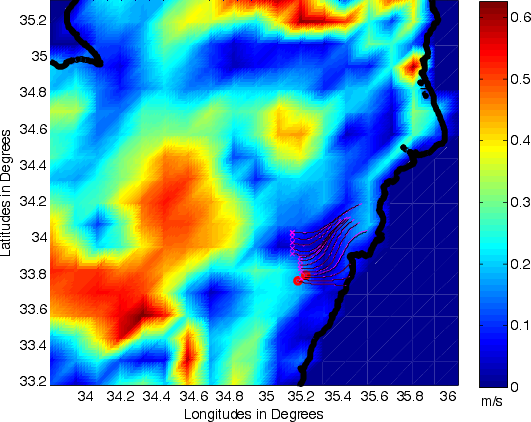
\includegraphics[width=\textwidth]{fig/After_L2pointw_win24_MEAN_color.png}
\end{columns}

Euclidian error on velocity field before and after assimilation.
\end{frame}

\begin{frame}{Results using real data}
Using the velocity field obtained by assimilating 2 drifters to
forecast the trajectory of a 3rd drifter (not used in the assimilation).\\
\vspace{3em}
\centering
\includegraphics[width=0.7\textwidth]{fig/ReconstructedCNRSExp_bmtogreen_2days_average_zoom.png}
\end{frame}


%%%%%%%%%%%%%%%%%%%%%%%%%
\begin{frame}
\frametitle{Summary of the method}
\begin{columns}[b]
\column{.5\textwidth}
\begin{figure}
\begin{tikzpicture}[
auto,
node distance = 0.4cm,
>=stealth',
weight/.style={rectangle,minimum height = .65cm, draw,fill=orange!20},
param/.style={rectangle,minimum height = .65cm, draw,fill=cyan!20},
neuron/.style={circle,minimum height = .65cm,draw,fill=magenta!20}]
\node [neuron] (plus) {$+$} ;
\node [neuron] (m) [above=of plus]{$\mathcal{M}$} edge [<-] (plus);
\node [neuron] (W) [left= of plus]{$\mathcal{W}$} edge [->] (m);
\node [param] (u) [below=of plus] {$u_b(t)$} edge [->] (plus);
\node[param] (w) [left=of u]{$w(t)$} edge[->] (W);
\node[weight] (a) [left=of w] {$a_w$} edge[->](W);
\node [param] (r) [left=of a] {$r_i(t)$} ;
\path [->,draw] (r) |- (m) ;
\node [weight] (du) [right=of u]{$\delta u$} edge [->] (plus);
\node [param] (y) [above=of m]{$r_i(t+1)$} edge [<-] (m);
\end{tikzpicture}
\caption{Physical network}
\end{figure}
\column{.5\textwidth}
\begin{onlyenv}<2>
\begin{block}{Summary}
\begin{itemize}
\item Very simple numerical model
\gooditem Makes use of the lagrangian information
\gooditem Improve eulerian velocity field
\pooritem No predictive power
\pooritem Uncertainty has to be evaluated
\pooritem Many "hyper-parameters"
\end{itemize}
\end{block}
\end{onlyenv}
\begin{onlyenv}<3>
\begin{figure}
\begin{tikzpicture}[
auto,
node distance = 0.4cm,
>=stealth',
weight/.style={rectangle,minimum height = .65cm, draw,fill=orange!20},
param/.style={rectangle,minimum height = .65cm, draw,fill=cyan!20},
neuron/.style={circle,minimum height = .65cm,draw,fill=magenta!20}]
\node [neuron] (plus) {} ;
\node [neuron] (m) [above=of plus]{} edge [<-] (plus);
\node [neuron] (R) [right= of plus] {} edge [->] (m);
\node [neuron] (W) [left= of plus]{} edge [->] (m);
\node[param] (w) [below=of plus]{$w(t)$} edge[->] (plus);

\node [param] (u) [right=of w] {$u_b(t)$} edge [->] (R);
%\node[weight] (a) [left=of w] {$a_w$} edge[->](W);
\node [param] (r) [left=of w] {$r_i(t)$} edge[->](W) ;
\node[weight] (we) [right= of u] {$\bf{W}$};
\path [->,draw] (we) -- (R) ;
\path [->,draw] (we) -- (plus) ;
\path [->,draw] (we) -- (W) ;
\path [->,draw] (we) edge [bend right] (m);

%\node [weight] (du) [right=of u]{$\delta u$} edge [->] (plus);
\node [param] (y) [above=of m]{$r_i(t+1)$} edge [<-] (m);
\end{tikzpicture}
\caption{Artificial neural networks (machine learning)}
\end{figure}
\end{onlyenv}
\end{columns}
\end{frame}


%%%%%%%%%%%%%%%%%%%%%%
\begin{frame}
\frametitle{Machine leaning for non-conventional observations}
\begin{block}{}
Internal representation of an image in a latent space (of reduced
dimension)
\end{block}
\begin{figure}
\centering
\begin{tikzpicture}
[
auto,
node distance = 0.5cm,
>=stealth',
image/.style={rectangle,minimum height = .65cm, draw,fill=blue!20},
latent/.style={rectangle,minimum height = .65cm, draw,fill=red!20},
model/.style={rectangle,minimum height = .65cm,draw,fill=green!20}]
\node[image] (out) {Ouput Image (= Input Image)} ;
\node[model] (nn2) [below=of out]{neural network} edge [->] (out);
\node [latent] (hid) [below=of nn2]{Internal representation of an image} edge [->]
(nn2);
\node[model] (nn1) [below=of hid]{neural network}edge[->] (hid);

\node [image] (in) [below=of nn1]{Input Image} edge[->] (nn1);
\visible<2> {\node (x) [right=of hid]{\footnotesize{pseudo-observation, state variables, ...}}
edge [<-] (hid);}
\end{tikzpicture}
\end{figure}
\end{frame}

%%%%%%%%%%%%%%%%%%%%%%%%%%%%
\begin{frame}
\frametitle{Application to the prediction of Total Suspended Matter}
\begin{figure}
\includegraphics[width=0.9\textwidth]{./fig/arch-tsm.png}
\caption{Proposed architechture to forecast total suspended matter}
\end{figure}
\rref[Brajard et al. (2017)]
\end{frame}

%%%%%%%%%%%%%%%%%%%%%%%%%%%%%
\begin{frame}
\frametitle{First results}
\begin{columns}
\column{.5\textwidth}
\begin{figure}
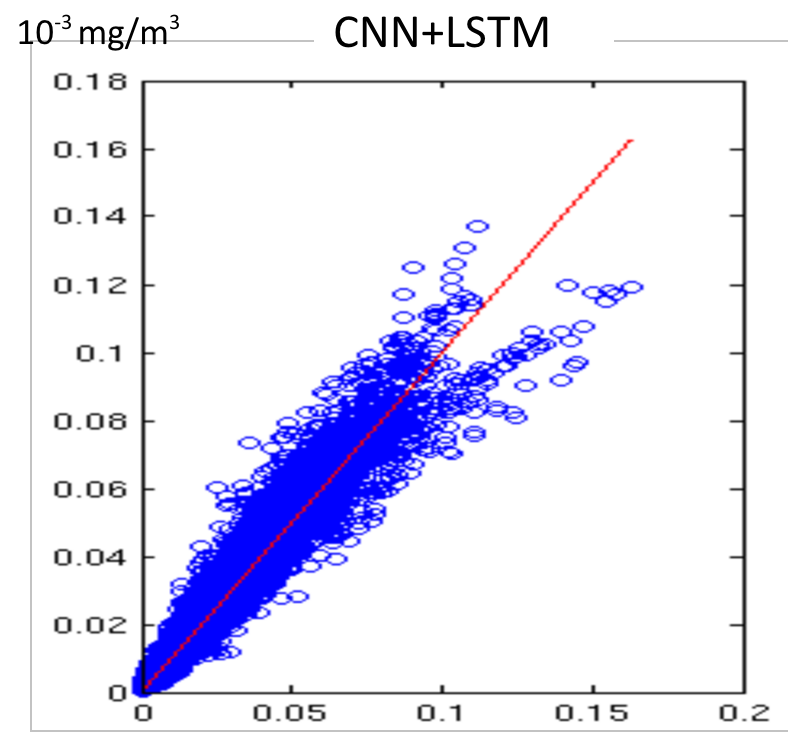
\includegraphics[width=0.9\textwidth]{./fig/scatter-tsm.png}
\caption{Scatter plot between real data and neural network prediction}
\end{figure}
\column{.5\textwidth}
\begin{figure}
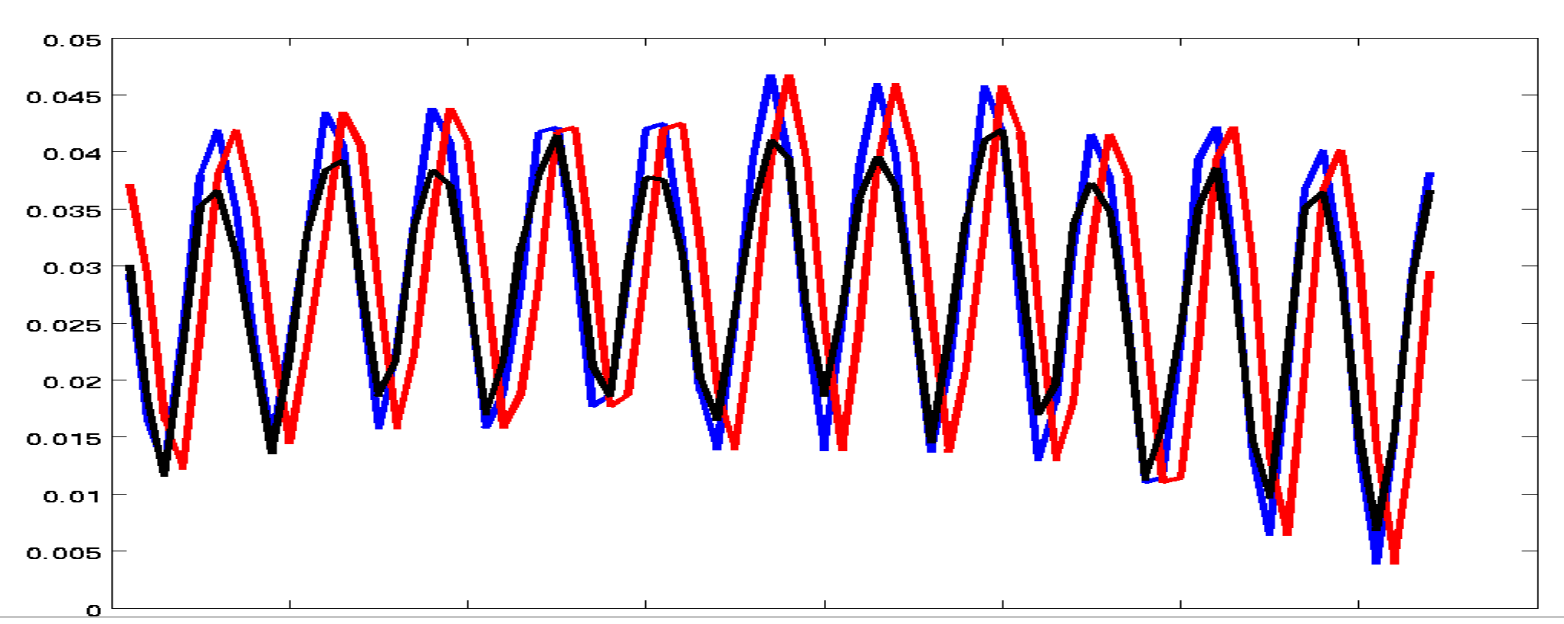
\includegraphics[width=0.9\textwidth]{./fig/serie-tsm.png}
\caption{Zoom of a time serie of the truth (in blue), the persistence
  model (in red) and the neural network prediction (in black)}
\end{figure}
\end{columns}
\end{frame}


%%%%%%%%%%%%%%%%%%%%%%
\begin{frame}
\frametitle{Conclusion}
\begin{block}{Bayesian data assimilation approach}
\begin{itemize}
\gooditem Some non-conventional data (e.g. lagrangian) can be handled
\gooditem Gives a theoritical framework (bayesian)
\pooritem A lot of a-priori assumption have to be made (e.g. error
statistics)
\pooritem Difficult when the model is badly known or too costly 
\end{itemize}
\end{block}
\begin{exampleblock}{Machine learning approach}
\begin{itemize}
\gooditem Very flexible method
\gooditem Can extract relevant structures in the image
\pooritem No theoritical framework
\pooritem Uncertainty difficult (but not impossible) to evaluate
\end{itemize}
\end{exampleblock}
\end{frame}


\end{document}